% you need to build with xelatex
\documentclass[t,aspectratio=169]{beamer}




\author{William O'Mullane}
\institute{AURA/Rubin Observatory}
\title{LSST Data Management }
\date{  \today}


\graphicspath{ {./images/} {./ETCcharts/} }

\def\pasp{PASP}

\usepackage{pdfpages}
\usepackage{amsmath,graphicx,marvosym}
\usepackage{tikz,multirow,array,colortbl,multimedia}
\usepackage{times,layouts}
\usepackage{tikz,hyperref}
\usetikzlibrary{positioning,arrows,shapes,decorations.shapes,shapes.arrows}
\usetikzlibrary{backgrounds,calc, shadows}
\usetikzlibrary{shapes.callouts}

\usepackage{graphicx}
\usepackage{natbib}
\usepackage{longtable}

\tikzstyle{flow}=[->, >=stealth', thick, shorten >=3pt, shorten <=3pt]

\def\aaps{A\&AS}           % Astronomy and Astrophysics Suplement
\def\aap{A\&A}             % Astronomy and Astrophysics
\def\ssr{Space~Sci.~Rev.}  % Space Science Reviews
\def\apj{ApJ}              % Astrophysical Journal
\def\aj{AJ}                % Astronomical Journal
\def\mnras{MNRAS}          % Monthly Notices of the RAS
\def\araa{ARA\&A}          % Annual Review of Astron and Astrophys
\def\nat{Nature}           % Nature
\def\apjl{ApJ}             % Astrophysical Journal, Letters

\def\degr{\hbox{$^\circ$}}
\def\arcmin{\hbox{$^\prime$}}
\def\arcsec{\hbox{$^{\prime\prime}$}}
\def\fs{\hbox{$.\!\!^{\rm s}$}}
\def\fdg{\hbox{$.\!\!^\circ$}}
\def\farcm{\hbox{$.\mkern-4mu^\prime$}}
\def\farcs{\hbox{$.\!\!^{\prime\prime}$}}
\def\sun{\hbox{$\odot$}}


%\newcommand{\bfvec}[1]{\mbox{$\bf#1$}}
%\newcommand{\citell}{\citeyear}
\newcommand{\citeds}{\citeyear}
%\newcommand{\citellp}{\citeyearpar}
%\newcommand{\citedsp}{\citeyearpar}
\providecommand{\secref}[1]{Section~\ref{#1}}
\providecommand{\appref}[1]{Appendix~\ref{#1}}
\providecommand{\partref}[1]{Part~\ref{#1}}
\providecommand{\tabref}[1]{Table~\ref{#1}}
\providecommand{\figref}[1]{Figure~\ref{#1}}
\providecommand{\eqnref}[1]{Eq.~\ref{#1}}
\providecommand{\reqref}[1]{Req.~\ref{#1}}
\providecommand{\actref}[1]{AI~\ref{#1}}


\newcommand{\jira}[1]{\href{https://jira.lsstcorp.org/browse/#1}{#1}}

\usepackage[backgroundTheme=LSST2017,
  fonts=false, colorlinks=false,
  footline=William O'Mullane $\bullet$ Rio \, Brazil  $\bullet$ September 2018,
  meeting= LSST Rio,
position={DM Project Manager}
]{LSST-beamer}


\title{LSST Data Management Overview  }
\date{25$^{th}$ September 2018}


\graphicspath{ {../../dm-docs/images}    }



\begin{document}

\maketitle
\section{Introduction}

\frame{\frametitle{ A little about myself}
	\vspace{-3pt}
\begin{itemize}
\item 1985ish started with BASIC on a  Commodore
\item 1993 MSc BSc Computer Science, University College Cork, Ireland
\item 1993 - 1997 Spacecraft Control Systems (C++), ESA ESOC  Germany
\item 1997 - 2001 Hipparcos, Integral, Planck, Gaia, Bepi-Sax  (C,Java,Oracle, HTM, HEALPix), ESA ESTEC Netherlands
\item 2001-2003 Commercial programming - some Astronomy (Java)
\item 2003-2005 The Johns Hopkins, SDSS and National Virtual Observatory (C,C\#,Java,Sqlserver)
\item 2005-2014 Gaia Astrometric Solution and Science Operations (Java, Oracle, Intersystems Cache)
\item 2012  PhD on Implementing the Gaia Astrometric Solution,  Barcelona University
\item 2014-2017 ESA SCI-OD division head - all science ground segments in development
\item 2017- LSST Data Management Project Manager (Python,C++), Deputy Project Manager for Software (control systems and IT)

\end{itemize}
}


\section{LSST status}
\frame { \frametitle{ LSST:uniform sky survey }
\begin{columns}
\column{0.45\textwidth}
\vspace {-0.3cm}
 \\
An optical/near-IR survey of half the sky in ugrizy bands to r~27.5 (36 nJy) based on 825 visits over  a 10-year period: {\em deep wide fast}.
%It’s about 5,000 sq. deg. per night, *twice*, on
%average. That is, about 1,000 visits per night on average. You return to
%the same position on the sky in about 3-4 nights (in any band). Btw, it’s
%a nice coincidence worth remembering that the total exposure time per
%position over 10 years (in all bands) is equal to about one observing night.
\begin{itemize}
\item 90\% of time  spent on  uniform survey: every 3-4 nights, the whole observable sky scanned twice per night
\item	~100 PB of data: about a billion 16 Mpix images, enabling measurements\\ {\color{cyan} for 40 billion objects! }
\end{itemize}
{\tiny see also \url{http://www.lsst.org} and \cite{2008arXiv0805.2366I}-arXiv:0805.2366}

\column{0.55\textwidth}
	 \includegraphics[width=0.9\textwidth]{images/coverage}\\
\vspace {-5pt}
{\bf 10-year simulation of LSST survey: number of visits in u,g,r band (Aitoff projection of eq. coordinates) }\\
\end{columns}

}
\frame { \frametitle{ LSST Camera }
\begin{columns}
\column{0.6\textwidth}
 \includegraphics[width=1.0\textwidth]{images/camera}
\column{0.4\textwidth}
 \\
\vspace {-3cm}
{\large \bf The largest astronomical camera:}
\begin {itemize}
\item 2800 kg
\item 3.2 Gpix
\end {itemize}
\end{columns}
}

\frame { \frametitle{ Site as imagined and in March 2019 }
\begin{columns}
\begin{column}{0.5\textwidth}
\vspace {7cm}
	\includegraphics[width=0.95\textwidth,trim=0cm 10cm 0 10cm,clip]{images/cerroRender}
\end{column}
\begin{column}{0.5\textwidth}
\\
	\includegraphics[width=0.95\textwidth,trim=0cm 0cm 5cm 0cm,clip]{images/cerroMar2019}
\end{column}
\end{columns}

}

\frame {\frametitle{  DM build and deploy - already challenging }
	\vspace{-1cm}
	\begin{columns}
		\column{0.4\textwidth}
		\begin{center}
			      \includegraphics[width=1.0\textwidth]{images/DMSDeployment}\\
		      \end{center}
		      \column{0.6\textwidth}
		       \\
		       \vspace{1cm}
		       DM must build everything to get LSST products (see \url{http://ls.st/dpdd})  to the users.
		       \begin{itemize}
			       \item large data sets (20TB/night)
			       \item complex analysis
			       \item aiming for small systematics
			       \item Science Alerts in under 2 minutes .. (aiming for 1 minute)
		       \end{itemize}
		       About $1\over{2}$  million lines of code (C++/python) all open source on github\\
		       \vspace{25pt}
		       {\tiny \bf diagram K.T. Lim}
	       \end{columns}
       }




\frame {\frametitle{  Data Backbone}
\begin{columns}
\column{0.45\textwidth}
      \includegraphics[width=1.0\textwidth]{images/DataBackbone}\\
\column{0.55\textwidth}
 \\
 One small box on the previous slide was Data Backbone.\\ That hides several things \\
 \begin{itemize}
	 \item Qserv - the LSST end user database
 \begin{itemize}
	 \item{\color{red} Custom Massive Parallel Processing (MPP) }
	 \item allow queries on $\approx 20$ Petabytes of tabular data
	\item $4 \times 10^{10}$ objects, $4 \times 10^{13}$ sources (observations)
 \end{itemize}
\item All the networks : we now have fiber to the mountain and from La Serena to NCSA (two routes)
 \end{itemize}
\vspace{25pt}
{\tiny \bf diagram K.T. Lim}
\end{columns}
}


\frame{\frametitle{Rubin Observatory Catalog 2035 }
Astronomy catalogs tend to be highly structured, tabular, somewhat predictable access.

\begin{columns}
\begin{column}{0.45\textwidth}

\begin{itemize}
\item Data, by DR11:
\begin{itemize}
\item  ~60T rows (mostly ForcedSource)
\item  ~10PB (mostly Source + ForcedSource + Object extra)
\end{itemize}
\item  Breakdown of most significant tables (rows x cols, storage):
\begin{itemize}
\item  Object: ~47B x 330, ~100TB
\item  Object extra: ~1.5T x 7,600, ~1.2PB
\item  Source: ~9T x 50, ~5PB
\item  ForcedSource: ~50T x 6, ~2PB
\end{itemize}
\end{itemize}
\end{column}
\begin{column}{0.55\textwidth}
\begin{itemize}
\item Get an object or data for small area - <10 sec
\item Scan through billions of objects - $\approx$ 1 hour
\item Deeper analysis (Object\_*) - $\approx$ 8 hours
\item Analysis of objects close to other objects -  $\approx$ 1 hour, even if full-sky
\item Analysis that requires special grouping - $\approx$ 1 hour, even if full sky
\item Source, ForcedSource scans - $\approx$ 12 hours
\item Cross match \& anti-cross match with external catalogs - $\approx$ 1 hour
\end{itemize}
\end{column}
\end{columns}
}


\frame{\frametitle{Qserv \tiny(slides from Fritz Muller) }

\begin{columns}
\begin{column}{0.6\textwidth}
\begin{itemize}
\item Shared-nothing MPP RDBMS (SQL, throughput, horizontal scaling)
\item  Spherical partitioning with overlap (near-neighbor self-joins)
\item  Shared scans (concurrent query load)
\item  Replicated data (resiliency)
\item  Fixed-purpose, dedicated hardware (cost, predictability)
\end{itemize}
\end{column}
\begin{column}{0.4\textwidth}

\includegraphics[width=0.90\textwidth]{images/spher}
	 Tesselation see  \cite{2001misk.conf..638O}
\end{column}
\end{columns}

Design optimized for use case + hardware efficiency \citeds{LDM-135}

Built on project at SLAC, leverage existing tech within Stanford (MariaDB, MySQL Proxy,
XRootD, Google protobuf, Flask)


100\% open source  \url{https://github.com/LSST/Qserv}
}

\frame{\frametitle{Shared Nothing Massively Parallel Processing }

\begin{columns}
\begin{column}{0.45\textwidth}

\includegraphics[width=1.1\textwidth]{images/distribute-combine}\\
		Recent scale tests: \url{https://dmtr-071.lsst.io}\\
		Perf and BigQuery: \citeds{Document-31100}
\end{column}
\begin{column}{0.5\textwidth}

\begin{itemize}
\item Ultimate target platform ~300 nodes in 2 international data-centers
\item	Development cluster (CC-IN2P3):
\begin{itemize}
\item  400 cores, 800 GB memory, 500 TB storage
\item  ~100 TB synthetic dataset on 2 x 25 nodes
\end{itemize}
\item Prototype Data Access Center (NCSA):
\begin{itemize}
	\item  500 cores, 4 TB memory, 700 TB storage
	\item  ~100 TB science dataset (SDSS Stripe 82 +
		WISE) on 30 nodes
	\item  + HSC reprocessing + GAIA DR2 coming up
\end{itemize}
\end{itemize}
\end{column}
\end{columns}
}




\frame {
  \frametitle{ Inevitably we must document ..  }

\begin{columns}
	\column{0.5\textwidth}
\begin{center}
   \includegraphics[width=0.9\textwidth,trim=0cm 0cm 0cm 0cm]{images/fops}\\
\end{center}
	\column{0.5\textwidth}
 \\
\vspace{1cm}
Gaia Flight Operations Procedures (FOP) paper copy in case the computers fail - could be useful!
\begin{center}
\vspace{5pt}
{\color{red} But we should avoid {\em write only} documents.}
\end{center}
\end{columns}
}




\frame{\frametitle{Guidelines,  tools,  conventions }
\begin{itemize}
    \item {\color{green} Its great having extensive guidelines - it was also something super on Gaia}
   \item \url{developer.lsst.io} is a full developer guide - everything from git commit messages to style guides for Python and C+.
   \item \url{pipelines.lsst.io} documents the main software release(s)
	\begin{itemize}
	\item worst of both worlds - it is a monolithic release  - but made up of > 120 git repos
	\item Still using \emph{in house} tools like EUPS \url{https://github.com/RobertLuptonTheGood/eups}
	\item moving toward conda-forge
	\item {\color{green} All open source (GPL) on github.com}
	\end{itemize}
\item  Language (spoken/written) and conventions are also super important
    \begin{itemize}
	    \item Single language projects  (like US or UK) fall more easily in the trap of \emph{believing} they speak  about the same topics because they speak language X.
	    \item {\color{blue} - on RubinObs we lack something foundational like \citeds{LL:BAS-003}}
    \end{itemize}

\end{itemize}
}


\frame {\frametitle{SDSS image }
	\begin{columns}
		\column{0.45\textwidth}
	      \includegraphics[width=1.0\textwidth]{images/SDSScosmos}\\
		      \column{0.55\textwidth}
		      \\
		       \vspace{1cm}
	       Nice colors \cite{2004PASP..116..133L}\\
	       $\approx  3.5 \arcmin$\\
		       \vspace{20mm}
	       {\tiny \bf{Image  Robert Lupton}}
	       \end{columns}
}
\frame {\frametitle{Hyper Suprime Cam (HSC) on Subaru }
\begin{columns}
      \column{0.45\textwidth}
		       \vspace{-20pt}
	      \includegraphics[width=1.0\textwidth]{images/HSCcosmos}\\
      \column{0.55\textwidth}
		       \\
		       HSC image (COSMOS) from g,r(1.5 hrs) ,i(3 hrs) PSF matched co-add ($\approx 27.5$)\\
		       Challenges:

\begin{itemize}
\item Unknown statistical distributions,   Truncated, censored and missing data, Unreliable quantities (e.g. unknown systematics and random errors)
\item PSF - short exposure - atmosphere dominated ?

\begin{itemize}
\item cosmic shear signal from weak lensing
\end{itemize}
\item Photometry  challenging - will Gaia help ..
\item Everything is blended!!
\end{itemize}
		{\tiny       Processed with  {\em LSST Stack} \url{https://pipelines.lsst.io/}\\
	        \bf{Image HSC collaboration,  Robert Lupton}}
\end{columns}
       }



\frame{\frametitle{Catalog extraction }
\begin{columns}
      \column{0.45\textwidth}
		       \vspace{-20pt}
	      \includegraphics[width=1.0\textwidth]{images/square/jupyterlab_nb}\\
      \column{0.55\textwidth}

\begin{itemize}
\item Identifying sources and disentangling them becomes more difficult as we have deeper images.
\item Left our typical Jupyter setup runs

\begin{itemize}
\item  Insrtrument signature removeval
\item  calibration
\item  source extraction
\item  overlay extracted information on cleaned image
\end{itemize}
\end{itemize}
\end{columns}
}



\section{Data Management Overview}

\frame {\frametitle{Organization}
\vspace{-0.6cm}
\begin{columns}
\column{0.7\textwidth}
\begin{center}
      \includegraphics[width=1.0\textwidth]{images/DmOrg}\\
\end{center}
\column{0.3\textwidth}

\vspace{0.1cm}

Welcome Leanne Guy  and thanks to Mario (who stays with us)!!\\
\vspace{0.2cm}
Welcome Michelle Butler  and thanks to  Don\\
\vspace{0.2cm}
Welcome Gabriele Comoretto.\\
\vspace{0.2cm}
Deputies John Swinbank (PM), Colin Slater (PS)  and Yusra AlSayyad (Pipelines)\\
\vspace{0.2cm}
{\color{red} Toughest thing in any project is communication.}
\end{columns}
}


%\frame  {\frametitle{DM Document Tree}
%\begin{center}
% \includegraphics[width=0.8\textwidth]{images/DocTree}
%\end{center}
%}

\frame{\frametitle{Verification is a Priority}
\begin{columns}
\column{0.70\textwidth}
 \includegraphics[width=1.0\textwidth]{images/DMMasterSchedule}
\column{0.30\textwidth}
\\
\vspace {-5.9cm}
Across all of LSST verification is a big topic right now.\\
\vspace {0.5cm}
DM is adopting a test driven schedule to better address this.\\
\vspace {0.5cm}
{\color{red} \citeds{LDM-503} Now generated from P6}
\end{columns}
}

\frame{\frametitle{Verification and Validation}
\textbf{Verification}: Have we built everything we are supposed to build?
\begin{itemize}
\item In line with the Project's System Engineering approach
\item Demonstrate that we cover all requirements on DM
\item \citeds{LDM-503} shows the DM verification matrix
\end{itemize}
\textbf{Validation}: Have we built the right thing and does it work as expected?
\begin{itemize}
\item Must tackle \textit{both} Scientific \textit{and} Operational Validation
\item Talking with with Commissioning Team: some \textit{rehearsals} will be joint
\end{itemize}

\begin{center}
\textbf{\citeds{LDM-503}} addresses DM's plans for verification \& validation.
\end{center}
}



\section{Data Management Recent Achievements }


\begin{frame}{Data Release Production }

\only<1-2>{
  \textbf{LDM-503-2: HSC (Hyper Suprime Cam) reprocessing milestone}

  \begin{itemize}

    \item{First (equal) post-replan, NSF-visible milestone hit by the DM project.}
    \item{Joint effort to reprocess (Data Facility team) and analyze (DRP team) HSC data
    under operations-like conditions}
    \item{Milestone successful: \citeds{DMTR-51}!}

  \end{itemize}
}

\invisible<1>{
  \textbf{``Warp Compare'' coadds}

  \begin{itemize}
    \item{New algorithm to robustly reject artifacts when coadding images.}
    \item{Now default for HSC processing; stack-wide default to be RFCed soon.}
  \end{itemize}

  \begin{center}
  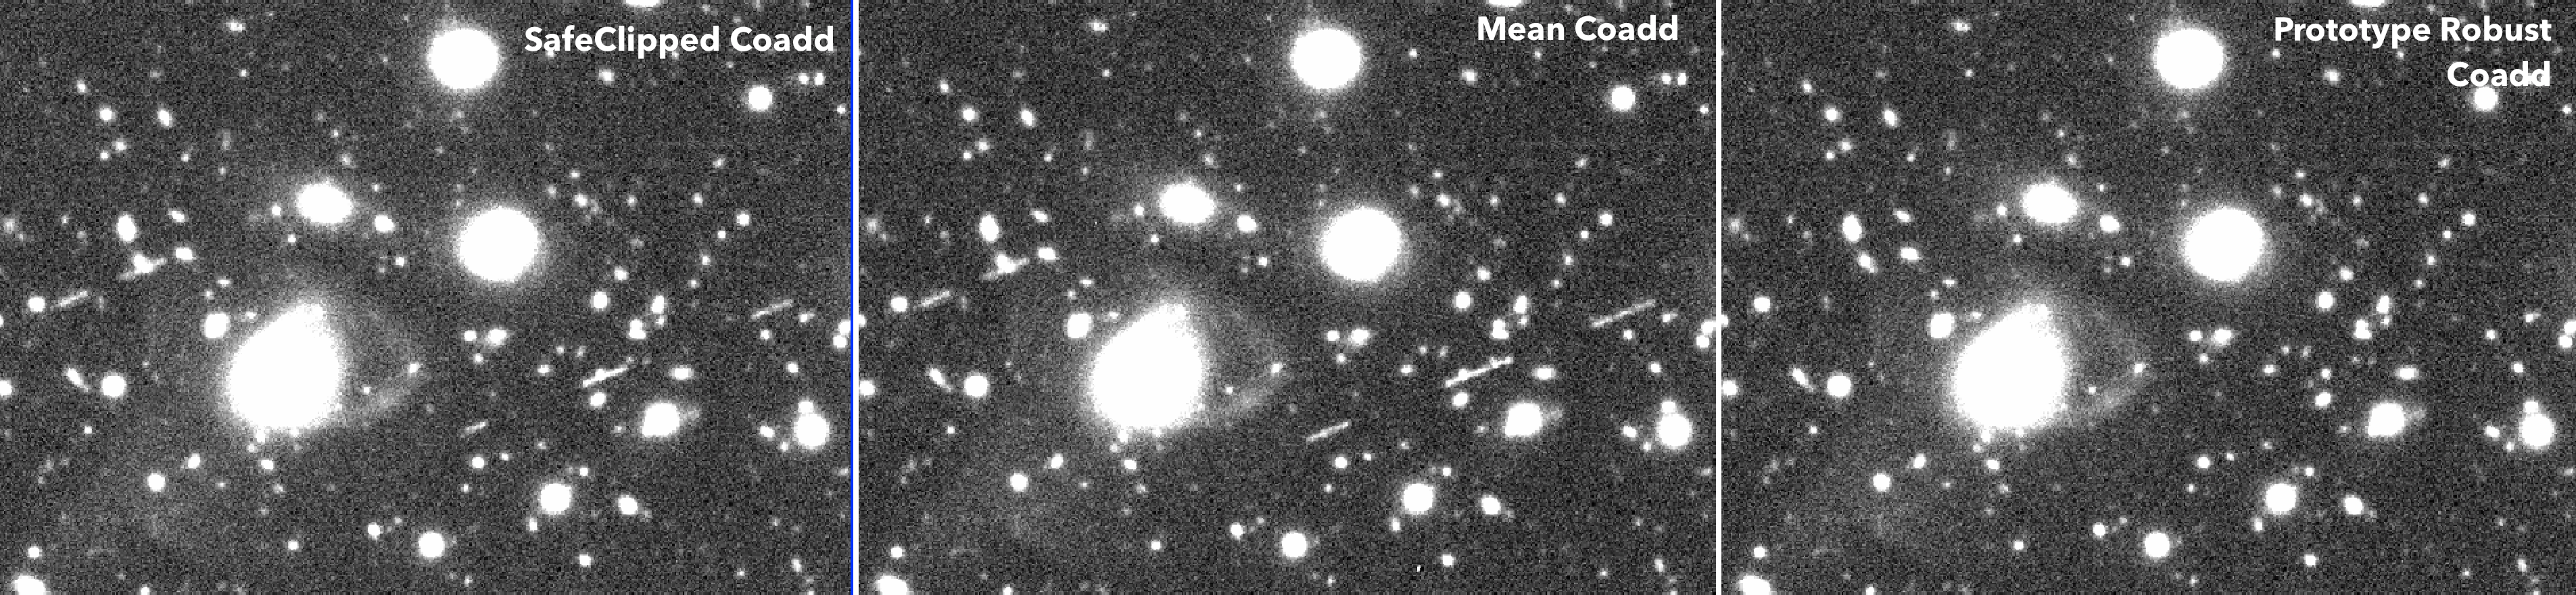
\includegraphics[width=0.5\textwidth]{figures/warpcompare.png}\\
  \tiny Figure: AlSayyad.
  \end{center}
}

\end{frame}


\frame {\frametitle{Alerts }

  \begin{itemize}
  \item \textbf{LDM-503-3: Alert generation milestone}
  \begin{itemize}

    \item First(equal) post-replan milestone  hit by the DM project \citeds{DMTR-53}!
    \item{Demonstrating a \textit{end-to-end} alert production pipeline.}

  \end{itemize}
\item Prototype alert distribution system using Kafka \& AVRO; benchmark results on \citeds{DMTN-028}.
\item   New MOPS (Moving Object)  linking algorithm under development and approach to Minor Planet Center \citeds{DMTN-087}.
  \end{itemize}


  \vspace{-0.5cm}
  \begin{columns}
    \begin{column}{0.72\textwidth}
      \begin{itemize}
	\item Jointcal replaces meas\_mosaic
      \begin{itemize}
        \item{Simultaneous astro- and photometric fitting to source lists derived
        from multiple images.}
        \item{The all new, much improved, more generic replacement for the
        HSC-specific meas\_mosaic.}
      \end{itemize}
      \end{itemize}
\tiny
\vspace{-5pt}
Figure shows the variation in photometric calibration not captured by single frame processing, normalized to 1.
\vspace{-5pt}
This demonstrates fine structure in photometry which Jointcal picks up but per-CCD processing doesn't catch.
\normalsize

    \end{column}

    \begin{column}{0.28\textwidth}
\vspace{-20pt}
      \begin{center}
        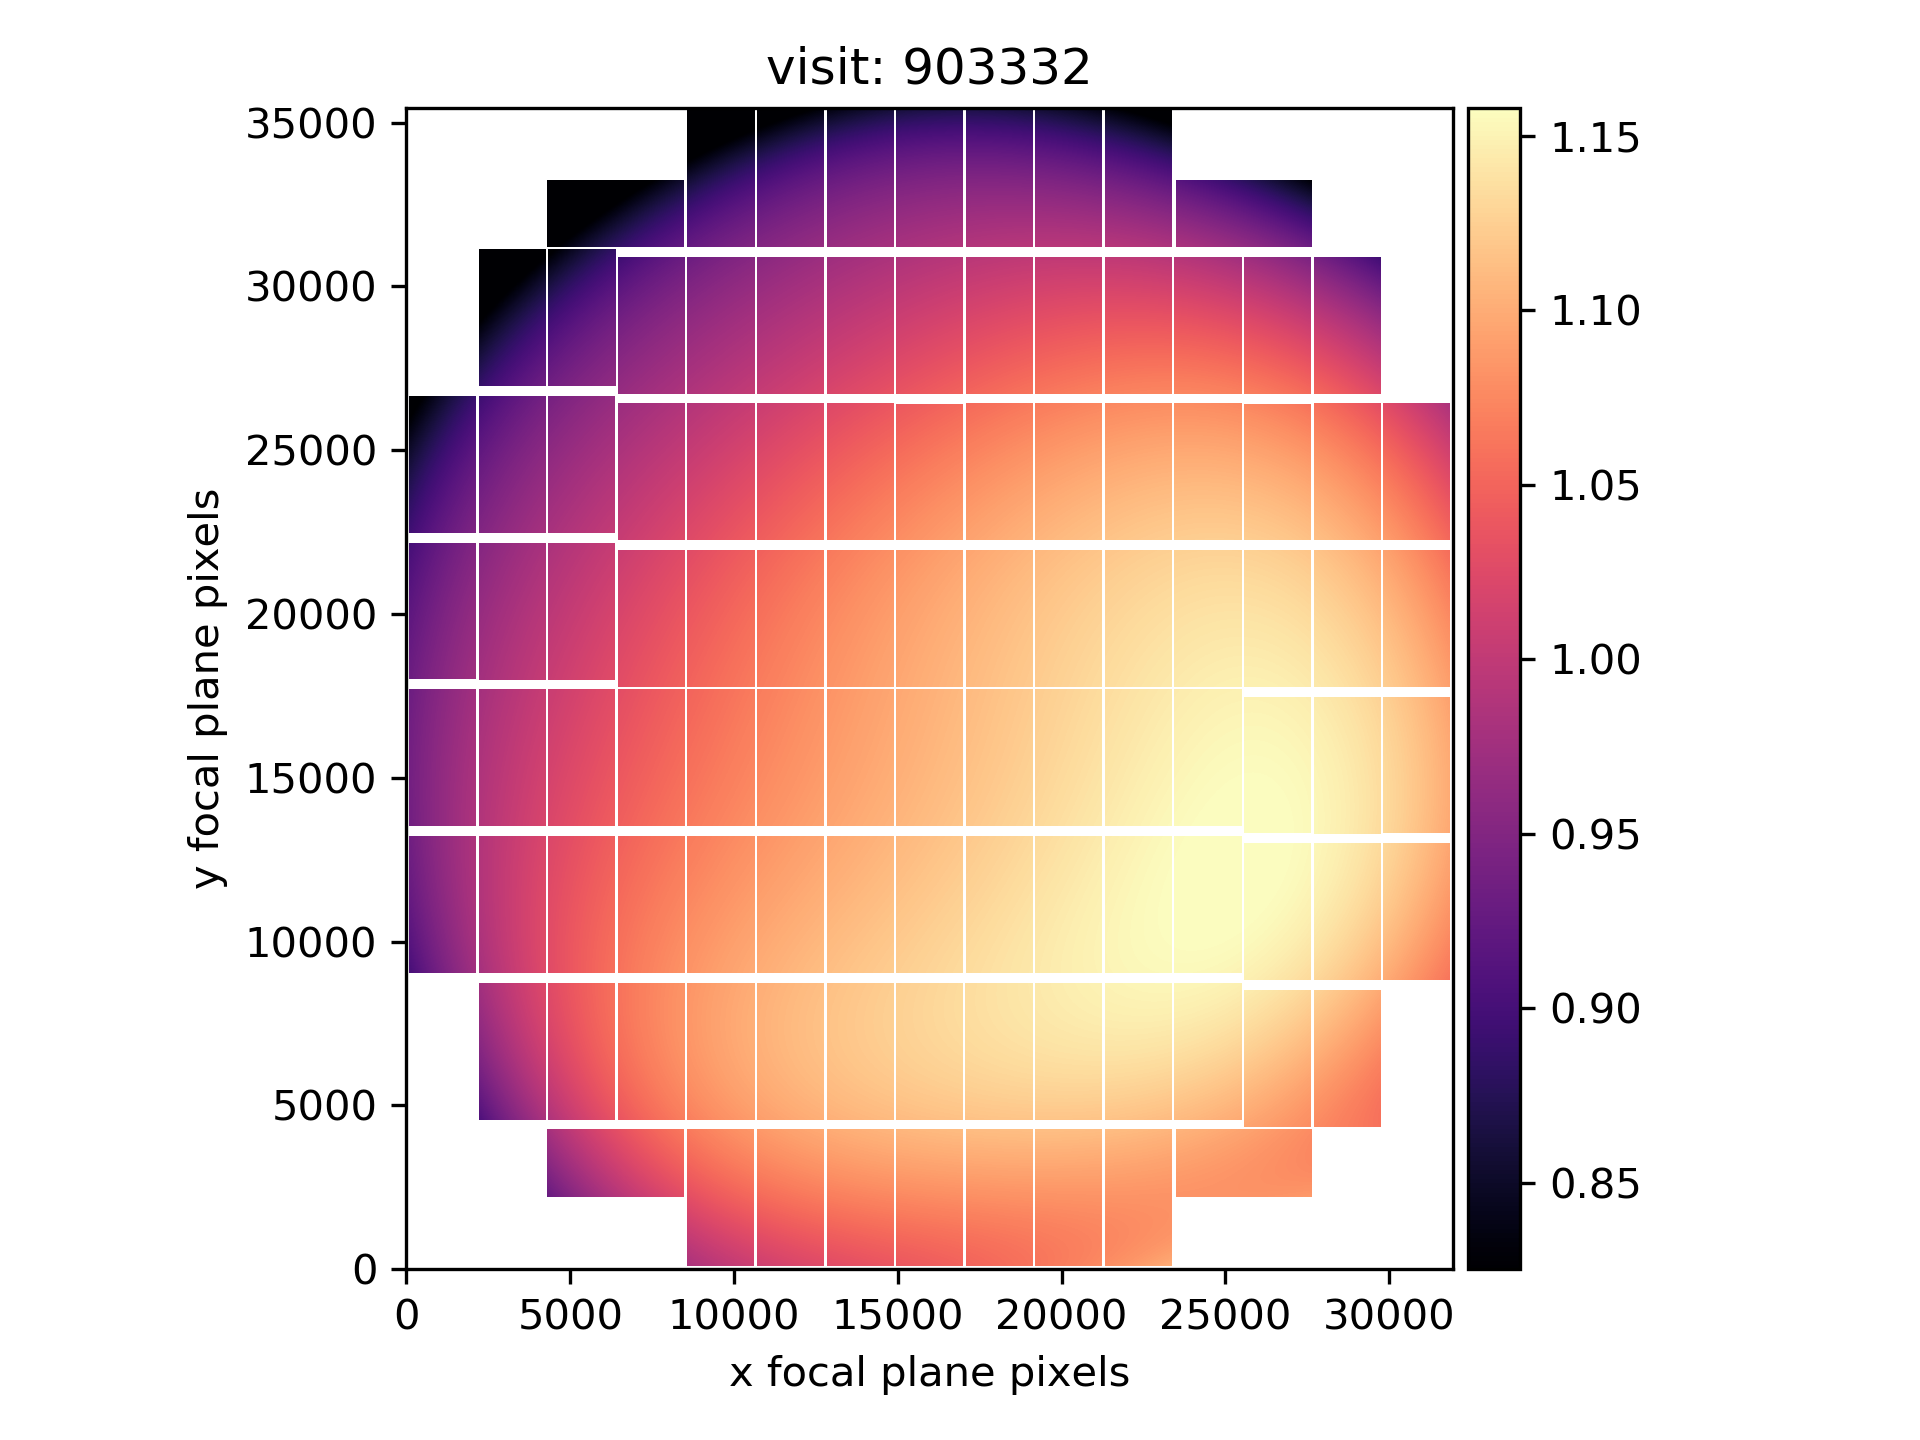
\includegraphics[width=1.0\textwidth]{figures/jointcal.png}\\
        \tiny Figure: Parejko.
      \end{center}
    \end{column}
  \end{columns}

}

\frame{\frametitle{Base \& Network: Fiber First Light }

\begin{columns}
\begin{column}{0.75\textwidth}
Successful transfer of digital data over LSST/AURA fiber optic networks from the Summit Site on Cerro Pachon to NCSA.  A set of 6 x 10 Gbps Network Interface cards on Data Transfer Nodes (DTN) configured with iPerf3 generated a sustained data rate of approximately 44 gigabits per second, over a period of 24 hours, exceeding the target of 40 gigabits per second.

\includegraphics[width=\textwidth]{net_firstlight}\\
\end{column}
\begin{column}{0.25\textwidth}
\vspace{0.3cm}
(\citeds{Document-28547})
\includegraphics[width=\textwidth]{net_firstlight_op}\\
\includegraphics[width=\textwidth]{net_firstlight_screen}
\end{column}
\end{columns}


}


\frame{\frametitle{Data Access Services }
\begin{columns}
    \begin{column}{0.6\textwidth}
        \begin{itemize}
            \item Catalog Database (Qserv) to 100 TB range
            \begin{itemize}
                \item Three 30-node clusters operating:
                \begin{itemize}
                    \item NCSA (PDAC): science dataset (Stripe 82 + AllWISE + NEOWISE)
                    \item CC-IN2P3 (2 x dev): synthetic dataset
                \end{itemize}
                \item 30\% DR1 KPM measurements \citeds{DMTR-17}
                        \item Deployment under Kubernetes
            \end{itemize}
	\item Gen 3 Data Butler and Supertask in progress
        \end{itemize}
    \end{column}
    \begin{column}{0.4\textwidth}
        \begin{center}
            
\includegraphics[width=\columnwidth]{figures/qserv-in2p3.png}
	{\tiny \bf IN2P3 Qserv Cluster - Fritz Muller}
        \end{center}
    \end{column}
\end{columns}
}



\frame{\frametitle{LSST Data Facility (NCSA) }
\begin{columns}
\begin{column}{0.5\textwidth}
\vspace{-6.3cm}
\begin{itemize}
\item  Observatory Operations Support (Level 1) Services

\begin{itemize}
\item Working within the LSST Systems Engineering Early Pathfinder group, developing and testing integration of T\&S, Camera, and DM service software via a series of early integration activities.
    \item Initial header service developed and configured for Camera subsystem and AuxTel use cases, ability to acquire pixel data and write FITS files, all commandable by OCS. Demonstrated on Level 1 Test Stand \citedsp{DMTR-61} and with Spectrograph in Tucson

\end{itemize}
\end{itemize}
\end{column}

\begin{column}{0.5\textwidth}
\includegraphics[width=1\textwidth]{EIA-341-Tucson-2018}\\
EIA-341 reading image from the spectrograph in Tucson July 2018
\end{column}
\end{columns}
}

\frame{\frametitle{Science Platform Vision to Reality (1.1) }
%\vspace{-10pt}
\vspace{-5pt}
Vision: \citeds{LSE-319} --- Design: \citeds{LDM-542} --- Test: \citeds{DMTR-51} at NCSA

\begin{columns}
\begin{column}{0.7\textwidth}
\includegraphics[width=1\textwidth]{images/psfnb}
\end{column}
\begin{column}{0.3\textwidth}
\vspace{-7cm}
\\
Portal/Browser\\
Notebooks\\
Web API\\
(Batch)\\
\hspace{-1.5cm} \includegraphics[width=1.3\textwidth]{images/firefly}\\
\hspace{0.1cm} {\tiny \bf Images Krughoff($\leftarrow$) and Wu ($\uparrow$)}
\end{column}
\end{columns}

}

\section{Conclusion}

\frame{\frametitle{Conclusion}
\begin{itemize}
\item New DM Project Management almost 1 year on the job !
\item We had a successful NSF/DOE Review in July 2017.
\item Will need to show verification for this summer
\item We move to implementation less experimentation - need to get things working
\item Starting  with AuxTel !
\item Thank you all for your continued efforts!

\end{itemize}
}

\frame {
  \frametitle{ The END }
\vspace{-0.3cm}
\begin{center}
 \includegraphics[width=0.4\textwidth]{images/SDSScosmos}
\hfill
 \includegraphics[width=0.4\textwidth]{images/HSCcosmos}\\
\vspace{-3.2cm}\hspace{0.7cm} \huge{\color{red} Questions?}\\
\vspace{+2.2cm}
\normalsize
{$\sim  3.5 \arcmin$ SDSS image   \hfill  HSC image (COSMOS)   \\\hfill \tiny g,r(1.5 hrs) ,i(3 hrs) PSF matched co-add ($\approx 27.5$)\\}

\vspace{-5pt}
{\tiny \url{http://www.lsst.org}} {\tiny \url{http://community.lsst.org}} \hfill
{\tiny Images:Lupton and HSC colaboration see also \cite{2004PASP..116..133L}}
\end{center}

}




\appendix

\section {Reference material}
\frame[allowframebreaks]{\frametitle{ Acronyms }
        \vspace{10pt}
        \tiny
        \addtocounter{table}{-1}
\begin{longtable}{|l|p{0.8\textwidth}|}\hline
\textbf{Acronym} & \textbf{Description}  \\\hline

AURA&Association of Universities for Research in Astronomy \\\hline
C&Specific programming language (also called ANSI-C) \\\hline
DM&Data Management \\\hline
ESA&European Space Agency \\\hline
ESAC&European Space Astronomy Centre (VilSpa) \\\hline
ESOC&European Space Operations Centre (ESA) \\\hline
ESTEC&European Space research and TEchnology Centre (ESA) \\\hline
HEALPix&Hierarchical Equal-Area iso-Latitude Pixelisation \\\hline
HTM&Hierarchical Triangular Mesh \\\hline
LSST&Large Synoptic Survey Telescope \\\hline
PhD&Doctorate in Philosophy \\\hline
SDSS&Sloan Digital Sky Survey \\\hline
TEC&Thermo-Electric Cooler \\\hline
USA&United States of America \\\hline
arcmin&arcminute, minute of arc (unit of angle) \\\hline
arcsec&arcsecond, second of arc (unit of angle) \\\hline
\end{longtable}

}

\frame[allowframebreaks]{\frametitle{ References }
       \tiny
       \bibliographystyle{lsst_aa}
       \bibliography{lsst,gaia_livelink_valid,refs,books,refs_ads}
       \normalsize

}



\end{document}
